\documentclass[]{report}

\usepackage[T1]{fontenc}
\usepackage[urw-garamond]{mathdesign}
\usepackage{garamondx}
\usepackage{amsmath, amsthm, amsfonts}
\usepackage[a4paper, total={5in, 8in}]{geometry}
\usepackage{tikz-cd} % used to draw commutative diagrams
\usepackage{graphicx}

% user defined commands go here
\newtheorem{theorem}{Theorem}[section]
\newtheorem{prop}[theorem]{Proposition}
\newtheorem{corollary}{Corollary}[theorem]
\newtheorem{lemma}[theorem]{Lemma}
\newtheorem{defn}[theorem]{Definition}
\newtheorem{examples}[theorem]{Example}
\newtheorem{exercise}[theorem]{Exercise}

\DeclareMathOperator\Spec{Spec}

\begin{document}

\title{%
    Introduction to Commutative Algebra: \\
    
    \large and affine algebraic varieties}
\author{Amal M}
\date{January 4, 2021}
\maketitle

\begin{abstract}

    The motivation for the study of algebraic geometry is how algebraic objects (rings of rational functions) are associated with varieties (zeros of polynomials). This subject florished during the second half of the twentieth century. Algebraic geometry allows us to study the geometry arising from algebraic objects. Core to the deeper understanding of this subject is an understanding of the subject of commutative algebra which studies commutative rings and their ideals and modules. The purpose of the present project is to gain an understanding of commutative algebra through solving exercises from Atiyah-MacDonald's book, Introduction to Commutative Algebra. The reading project comprised of the study of the theory of rings and modules, their tensor product and exact sequences of rings and modules. The project concluded with a proof of the Going-Up Theorem.

\end{abstract}

\tableofcontents
\newpage

\chapter{Introduction}

The purpose of the current project is to give an understanding 
to the reader of how commutative algebra is used to define the basic
objects of algebraic geometry. Algebraic Geometry is the study of
the geometric properties of the solution set of polynomial equations
in arbitary variables. For this purpose it is useful to confine the 
discussion to algebraically closed fields $k$ and the polynomial ring
$k[x_1,\cdots,x_n]$. We define \textit{affine n-space} over the algebraically closed field $k$ as $k^n$ and denote it by $\mathbb{A}^n_k$.

\begin{defn} The algebraic variety \cite{vakil145} in the affine space $\mathbb{A}^n_k$ of a set $S$ of polynomials $f\in k[x_1,\cdots, x_n]$, is a subset $V(S)\subseteq \mathbb{A}^n_k$ cut out by the set of mutual zeros of all the polynomials in the set $S$.  
    $$V(S) = \{x = (x_1,\cdots,x_n) \in \mathbb{A}^n_k : f(x) = 0 \text{ for all } f \in S\}.$$
\end{defn}

The affine variety is not the only example of a variety. The projective variety defined over projective spaces $\mathbb{P}^n_k$ is another example of an algebraic variety.

The solution set or \textit{locus} of solutions of polynomials of degree one are discrete points in $k$. But over $k^2$ the \textit{locus} are curves. For example, the solution of the elliptic curve given by the polynomial equation in $\mathbb{R}[x,y]$ in $\mathbb{R}^2$  
    $$y^2 = x^3 - 3x + 5$$
    is a curve (Fig 1.). The question then arises: \textit{what does the solution set of a set of polynomials in $k^3$ look like? What about $k^n$?} This is same asking the question: \textit{what does an affine algebraic variety in $\mathbb{A}^n_k$ look like?} We may go further by demanding: \textit{what is the topology of the affine algebraic variety?} (The answer is called the \textit{Zariski Topology}, which we shall get to in due time.)

    Once we have an affine algebraic variety we may define functions on them and we may define functions from one algebraic variety to another. Thus we start to do the usual mathematical \textit{shtick} on affine varieties.

    To answer the proposed questions we need to know the properties of an affine algebraic varieties. For example: \textit{what is so algebraic about an affine algebraic variety?} The answer is that we may consider every \textit{affine algebraic variety} to be some \textit{finitely generated nilpotent-free $k$-algebra $A$}. To know what each of these terms means we first need some commutative algebra. The purpose of this article is to explain these terms and give a brief introduction to Algebraic Geometry focusing only on affine algebraic varieties.

    The exposition is based on the knowledge gained after spending many hours working out the exercises contained in \cite{atiyah1}. I would advise anyone thinking about learning algebraic geometry to start there and work out those exercises themselves.  

    We divide the article into four sections. In the first section we introduce the \textit{prime spectrum} of a ring $A$, $X = \Spec(A)$ by which we denote the set of all prime ideals of $A$. We endow this space $X$ with a topology called \textit{the Zariski Topology}.

    In the next section, we introduce \textit{modules}, which are a sort of generalised vector spaces and \textit{algebras}, which are modules on rings, and we define the tensor product on a collection of such \textit{modules}. Then we discuss a particular sort of structure that can be given to a collection of modules called \textit{the direct limit} -- a term loaned from Category Theory. 

    In the third section we introduce the \textit{rings of fractions} of modules and the concept of \textit{localization} which we use in the formulation of a sort of structure called \textit{presheaf} and \textit{sheaf}. We also introduce the \textit{constructible topology} and the precise condition under which this topology is equivalent to the \textit{Zariski Topology} on $\Spec(A)$. 

    In the final section we introduce integral dependence, that is elements of rings that are integral over a subring and discuss the proof of the Going-Up Theorem, one of the two well known theorems of Cohen-Seidenberg. 

    % Start by giving an overview of the table of content

\begin{figure}
  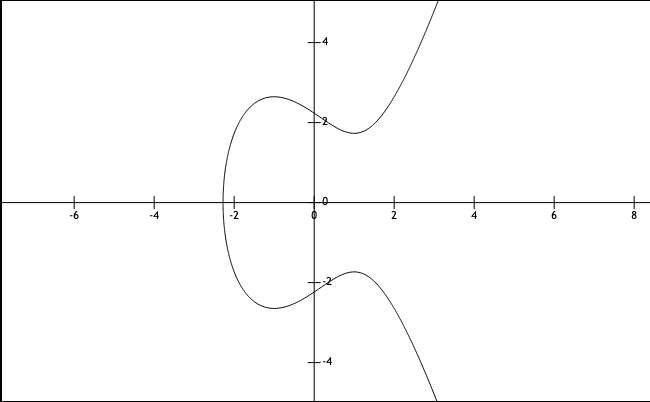
\includegraphics[width=\linewidth]{img/ell_curv1.png}
  \caption{Fig 1.}
  \label{fig:ell_curv1}
\end{figure}

\chapter {The Zariski Topology}

In commutative algebra what we generally call a \textit{ring} is a ring with unity, i.e, $1\in A$. So from now on, when we say ring we mean a set $A$ with two binary operations on it's elements $a + b \text{ and } a\dot b$, for all $a,b\in A$ such that A is an abelian group with respect to addition and multipication is associative and distributive over addition and $1\in A$ is the unique identity element.

A \textit{unit} in a ring $A$ is an element $x\in A$ such that there is another element $y\in A$ so that $xy = 1$. A ring in which every element is a \textit{unit} is called a \textit{field}. 

An element $x\in A$ is a \textit{nilpotent} element if $x^n = 0$ for some $n>0$. An element $x$ is an \textit{idempotent} element if $x^2 = x$. 

If we are given a group we know that if we quotient it by a normal subgroup we obtain another group and that the kernal of a group homomorphims is always a normal subgroup. Similarily rings have \textit{ideals}. Using \textit{ideals} can form a quotient ring and we have the fact that the kernal of every ring homomorphim is an ideal. 

\begin{defn}
    A subset $\mathfrak{a} \subseteq A$ is called an \textit{ideal} of $A$ if $\mathfrak{a}$ is an additive subgroup and it has the property, $y\in \mathfrak{a}$ and $x\in A$ implies $xy\in \mathfrak{a}$.
\end{defn}

Once we undersand what an ideal is we can define a \textit{prime ideal} of $A$ which is an ideal $\mathfrak{p}$ of $A$ with the property that $xy\in \mathfrak{p} \implies x \in \mathfrak{p} \text{ or } y\in \mathfrak{p}$. Similarily an ideal $\mathfrak{m}$ in A is \textit{maximal} if $\mathfrak{m} \neq (1)$ and if there is no ideal $\mathfrak{a}$ such that $\mathfrak{m\subset a\subset} (1)$. If we understand that given an ideal $\mathfrak{a}$ of a ring $A$ we can form the quotient ring $A/\mathfrak{a}$, we can look at the following proposition given without proof

\begin{prop}
    $$\mathfrak{p} \text{ is prime } \Leftrightarrow A/\mathfrak{p} \text{ is an integral domain }$$
    $$\mathfrak{m} \text{ is maximal } \Leftrightarrow A/\mathfrak{m} \text{ is a field }$$
\end{prop}

Therefore every \textit{maximal ideal} is a \textit{prime ideal} but the converse is not true in general. The reason prime ideals and maximal ideals are so important is because they have "nice" properties when we transport them across ring homomorphims. For example given a ring homomorphim $f:A\rightarrow B$ and a prime ideal $\mathfrak{q}\subset B$ the set $f^{-1}(\mathfrak{q})$ is a prime ideal  $\mathfrak{p}\subset A$. This result will be useful later on. Meanwhile we move onto the other memebers of \textit{ring theory}. 

A ring with just one \textit{maximal} ideal $\mathfrak{m}$ is called a \textit{local ring}. The quotient ring $k = A/\mathfrak{m}$ which is a field, is called the \textit{residue field} of $A$. 

\begin{defn}
    The radical of an ideal $\mathfrak{a}\subset A$ is another ideal 
    $$r(\mathfrak{a}) = \{x\in A: x^n\in \mathfrak{a} \text{ for some } n>0\}$$
\end{defn}

We can show that the \textit{radical} of an ideal is the intersection of all prime ideals that contain that ideal. If $x$ is an element of $\mathfrak{a}$ and if $x$ is any power of an element then that element belongs to the \textit{radical}. So the \textit{radical} is a way to associate elements related to $\mathfrak{a}$ by it's power. That is, if $f^n\in \mathfrak{a}$ then by definition of an ideal all the powers of $f$ higher than $n$ also belongs to $\mathfrak{a}$, the \textit{radical} ideal includes \textit{lower powers} of $f$ such as $f^{n-2}, f^{n-5}$ and so on. So we can have all powers of $f$ in $r(\mathfrak{a})$. 

We just need to define one more concept before we can move on to define the \textit{prime spectrum} of a ring. 

\begin{prop}
    The set $\mathfrak{N}$ of all nilpotent elements in a ring A is an ideal and $A/\mathfrak{N}$ has no nilpotent element $\neq 0$. \cite{atiyah1}
\end{prop}

The \textit{nilradical} of a ring $A$ has the property that it is equal to the intersection of all the prime ideals of $A$. It's worth asking the question: \textit{What is the intersection of all maximal ideals of $A$?}. The answer is precisely the \textit{Jacobson ideal} of $A$ denoted by $\mathfrak{R}$. It has the following property

\begin{prop}
    $x\in \mathfrak{R} \Leftrightarrow 1-xy$ is a unit in A for all $y\in A$. \cite{atiyah1}
\end{prop}



\section{Prime Spectrum}
\section{Zariski Topology}
\section{Irreducible Spaces}
\section{Affine Algebraic Varieties}


\chapter{Tensor Product and Direct Limits}
\section{Tensor Product}
\section{Flatness}
\section{Direct Limit}

\chapter{Sheaf and Presheaf}
\section{Support}
\section{Presheaf}
\section{Sheaf}
\section{Constructible Topology}
\section{Absolute Flatness}

\chapter{The Going-Up Theorem}

\begin{thebibliography}{9}

\bibitem{vakil145}
    Ravi Vakil,
    \textit{Math 145: Algebraic Geometry}

\bibitem{atiyah1}
    Atiyah-Macdonald, 
    \textit{Introduction to Commutative Algebra}
\end{thebibliography}

\end{document}
